Créer un compte ChromaCase vous permet de sauvegarder et suivre votre historique et progression.

À partir de la page d’accueil, il faut cliquer sur le bouton \textit{Sign up for free} (Voir Capture \ref{fig:signup}).

\begin{figure}[H]
	\begin{subfigure}[b]{0.7\textwidth}
		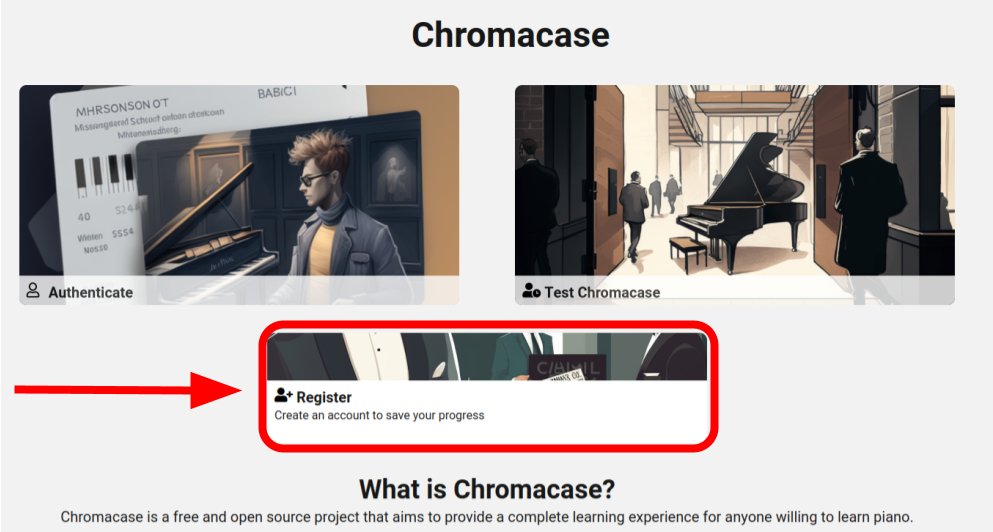
\includegraphics[width=\linewidth]{../\dir/guide/auth/register.png}
		\caption{Version navigateur}
	\end{subfigure}
	\begin{subfigure}[b]{0.25\textwidth}
		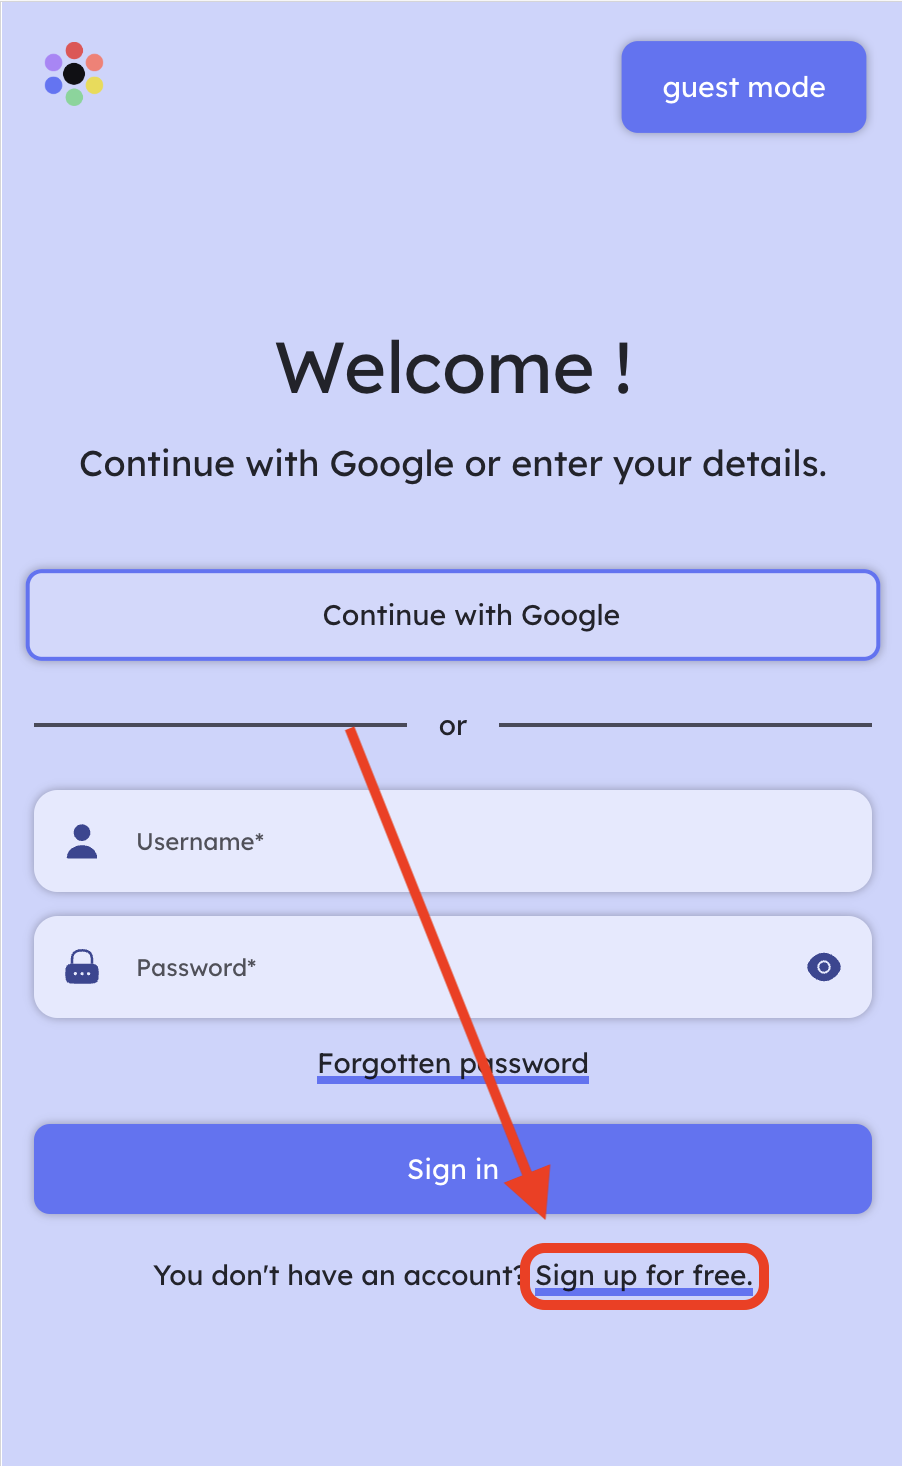
\includegraphics[width=\linewidth]{../\dir/guide/auth/register-mobile.png}
		\caption{Version mobile}
	\end{subfigure}
	\caption{Créer un compte}
	\label{fig:signup}
\end{figure}

Une fois rendu sur le formulaire, saisissez votre nom d’utilisateur, votre email ainsi que votre mot de passe.
Ce dernier doit contenir au moins six caractères, incluant au moins une majuscule, une minuscule et un chiffre.

Une fois le formulaire rempli, cliquez sur le bouton “Sign Up” (Voir Capture \ref{fig:signup-form}).

\begin{figure}[H]
	\begin{center}
		\begin{subfigure}[b]{0.7\textwidth}
			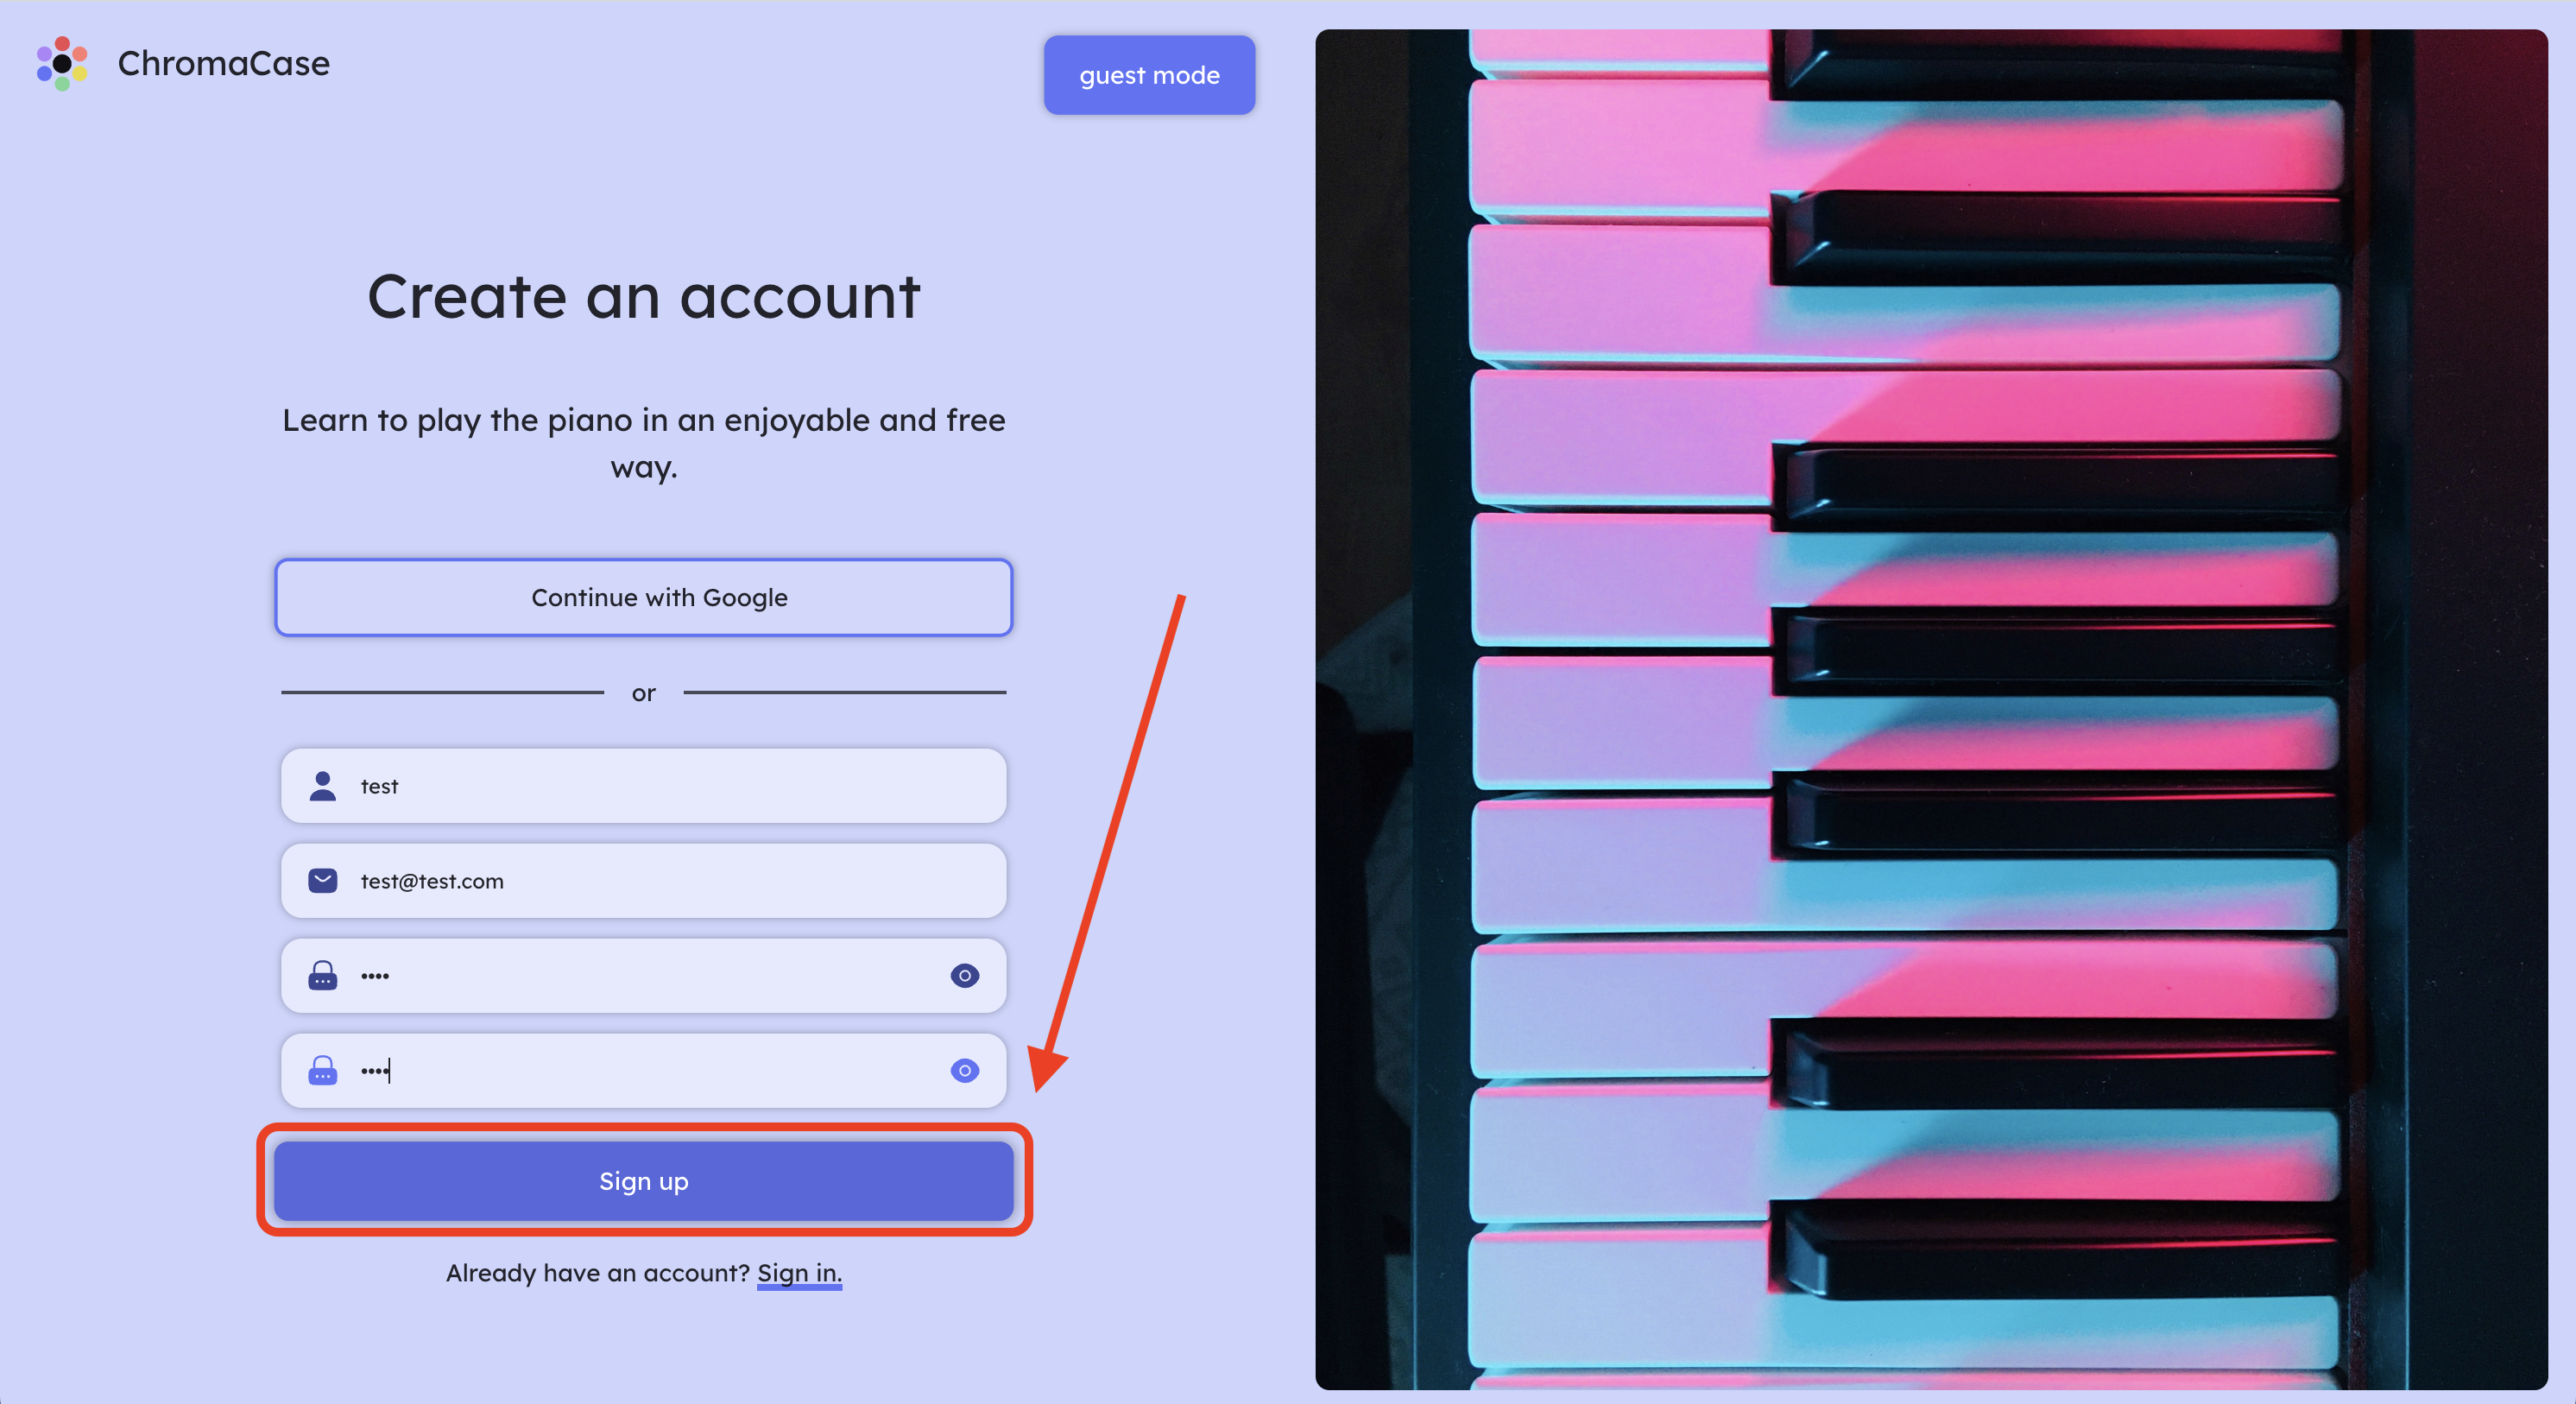
\includegraphics[width=\linewidth]{../\dir/guide/auth/signup.png}
			\caption{Version navigateur}
		\end{subfigure}
		\begin{subfigure}[b]{0.25\textwidth}
			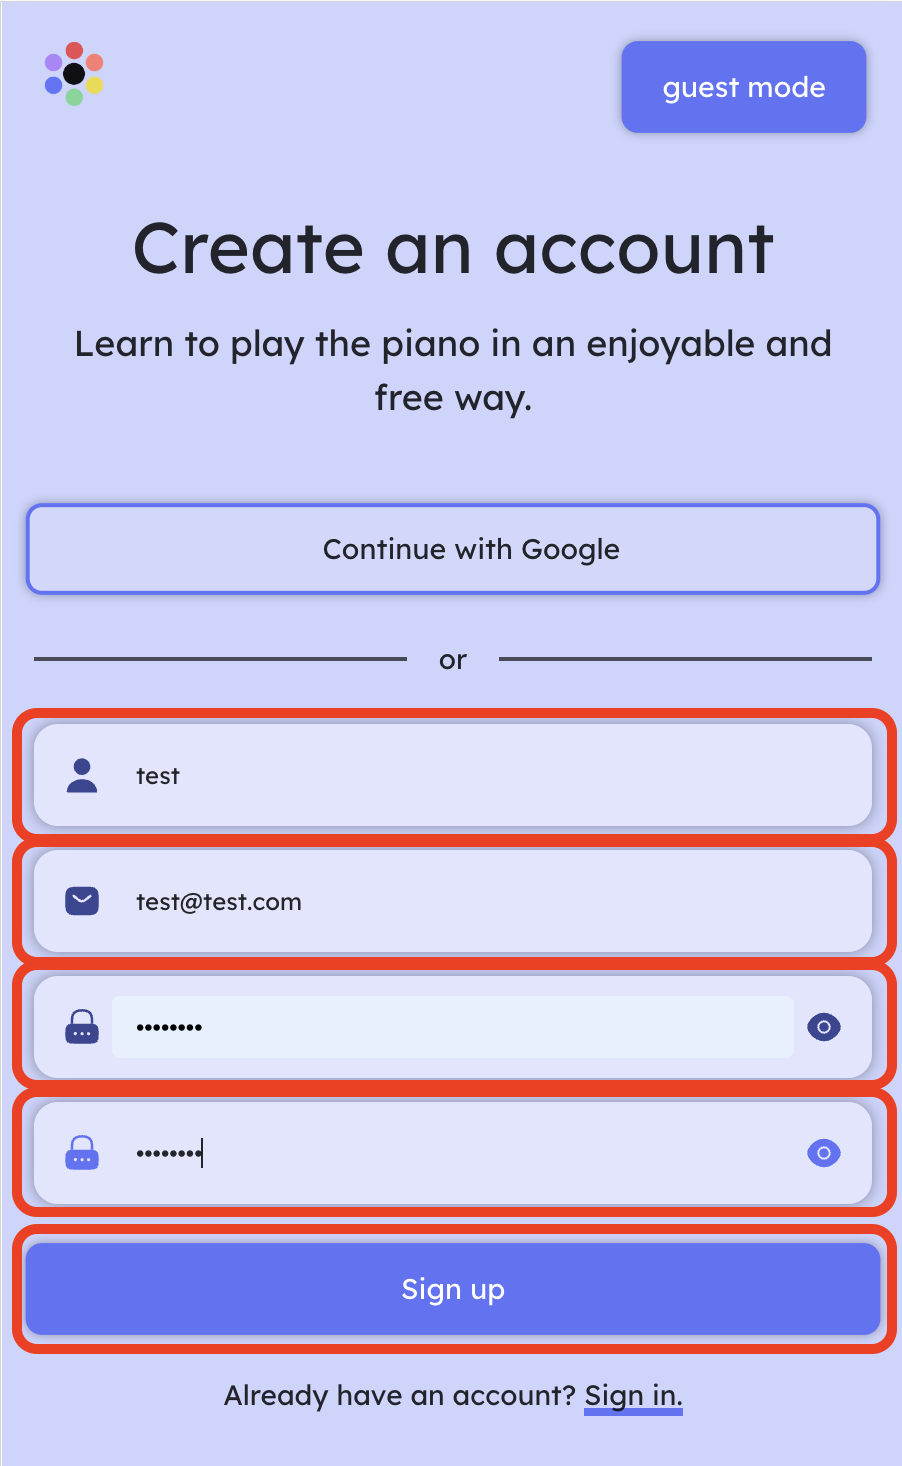
\includegraphics[width=\linewidth]{../\dir/guide/auth/signup-mobile.png}
			\caption{Version mobile}
		\end{subfigure}
		\caption{Valider la création d'un compte}
		\label{fig:signup-form}
	\end{center}
\end{figure}

Votre compte sera créé et vous serez redirigé.e sur votre page personnelle!